\section{Bildaufnahme}

\begin{defi}[Kamera]{Schema}

    \centering
    \includegraphics[width=0.8\textwidth]{figures/kamera-schema.pdf}
\end{defi}

\begin{defi}[Kamera]{Filter}
    % TODO: https://de.wikipedia.org/wiki/Filter_(Fotografie) 
    \emph{Filter} sind optische Elemente eines bildgebenden Systems, die in der Fotografie meist vor dem Objektiv der Kamera angebracht werden.

    Sie verändern das einfallende Licht bereits vor dem Objektiv und Film oder Bildsensor.
    Sie werden verwendet, um optische Effekte positiv zu korrigieren oder spezielle Effekte zu erreichen.

    Während optische Filter vor der Erfindung der Digitalfotografie ein wichtiges Element der analogen Fotografie waren, spielen sie mittlerweile durch immer bessere Kamerasoftware und spätere Bearbeitungsmöglichkeiten eine zunehmend geringere Rolle -- mit wenigen Ausnahmen wie etwa Polfiltern und Neutraldichtefiltern.
\end{defi}

\begin{example}[Kamera]{Filter}
    % TODO: https://de.wikipedia.org/wiki/Filter_(Fotografie) 
    Die meisten Filter reflektieren einen Teil des einfallenden Lichtes, so dass weniger Licht das Objektiv erreicht.
    Diese Belichtungsreduktion wird durch den Filterfaktor angegeben.
    Dieser ist meist auf der Fassung des Filters angegeben.

    Wichtige Filter sind z. B.:
    \begin{itemize}
        \item \emph{Polarisationsfilter}
        \item \emph{UV-Sperrfilter} und Skylightfilter
        \item \emph{Farbfilter} bzw. \emph{Konversionsfilter} und \emph[Korrekturfilter] (Rot, Grün, Blau, Gelb etc.)
        \item \emph{optische Spezialfilter}
        \item \emph{Infrarot-Sperrfilter}
        \item \emph{Neutraldichtefilter} (kurz ND-Filter, meist auch als Graufilter bezeichnet)
        \item \emph{Effektfilter} (z. B. Stern-, Regenbogen- und Farbverlauffilter)
    \end{itemize}
\end{example}

\begin{defi}[Kamera]{Objektiv}
    % TODO: https://de.wikipedia.org/wiki/Objektiv_(Optik) 
    Ein \emph{Objektiv} ist ein sammelndes optisches System, das eine reelle optische Abbildung eines Gegenstandes (Objektes) erzeugt. Es ist die wichtigste Komponente abbildender optischer Geräte, zum Beispiel von Kameras, Ferngläsern, Mikroskopen, Projektoren oder astronomischen Teleskopen.

    Das einfachste Objektiv ist eine einzelne Sammellinse, wie sie um 1608 die ersten Fernrohre hatten.
    Bestandteile eines Objektivs können jedoch sowohl Linsen, als auch Spiegel oder (seltener) Beugungsgitter sein, die sich je nach Einsatzzweck in einem oder mehreren Tuben befinden, die innen geschwärzt und gerippt sind, um Streulicht zu reduzieren.

    Die Hauptmerkmale eines Objektivs sind dessen Brennweite, die für einen gegebenen Objektabstand den Abbildungsmaßstab bestimmt, und die Apertur (freie Öffnung der Frontlinse).

    Weitere wichtige Eigenschaften sind die Abbildungsqualität, die durch eine geeignete Kombination mehrerer Linsen unterschiedlicher Brechungsindizes, Dicken und Krümmungsradien bestimmt wird und zur Verringerung optischer Abbildungsfehler dient, sowie die Streulichtempfindlichkeit, die möglichst gering sein sollte.
    Die Streulichtempfindlichkeit ist vor allem bei Gegenlicht wichtig und kann durch geschwärzte Blenden vermindert werden.

    Weitere Eigenschaften sind die fotografische Lichtstärke (Öffnungsverhältnis) und die Naheinstellgrenze, welche bestimmt, wie nah man an das Motiv \enquote{herangehen} kann (Makro).
\end{defi}

\begin{defi}[Kamera]{Linse}
    Als \emph{Linsen} bezeichnet man in der Optik transparente Scheiben, von deren zwei Oberflächen wenigstens eine -- meistens sphärisch -- gekrümmt ist.

    Durchgehendes Licht wird an den Oberflächen gebrochen und zur Mitte des Lichtbündels abgelenkt (gesammelt, Sammellinse) oder nach außen gestreut (Zerstreuungslinse).
    Eine konvexe Oberfläche sammelt, eine konkave Oberfläche zerstreut das Licht.

    Die Größe des Bildes wird von der \emph{Brennweite} $f$ der Linse und dem Abstand $g$ zwischen Gegenstand und Linse bestimmt.

    \centering
    % TODO: https://de.wikipedia.org/wiki/Linsengleichung 
    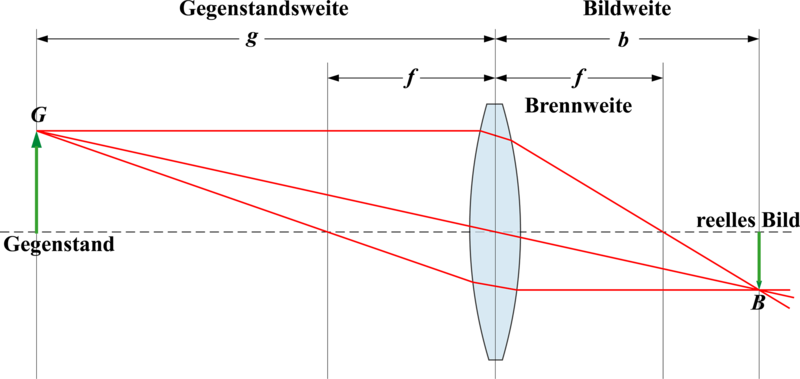
\includegraphics[width=0.6\textwidth]{figures/linse.png}
\end{defi}

\begin{defi}{Abbildungsmaßstab}
    % TODO: https://de.wikipedia.org/wiki/Abbildungsmaßstab 
    Der \emph{Abbildungsmaßstab} $\beta$ ist definiert als das Verhältnis zwischen der Bildgröße $B$ der optischen Abbildung eines Gegenstandes und dessen realer Objektgröße $G$.
    Alternativ kann der Abbildungsmaßstab auch über das Verhältnis von Bildweite $b$ zur Gegenstandsweite $g$ bestimmt werden:
    \[
        \beta = \frac{B}{G} = \frac{b}{g}
    \]
\end{defi}

\begin{defi}{Linsengleichung}
    % TODO: https://de.wikipedia.org/wiki/Linsengleichung 
    Die \emph{Linsengleichung} gibt bei einer optischen Abbildung mittels einer Linse die Beziehung zwischen Gegenstandsweite $g$, Bildweite $b$ und Brennweite $f$ an.
    Sie lautet:
    \[
        \frac{1}{f} = \frac{1}{b} + \frac{1}{g}
    \]
\end{defi}

\begin{defi}[Kamera]{Blende}
    % TODO: https://de.wikipedia.org/wiki/Blende_(Optik) 
    \emph{Blenden} sind in der Optik Vorrichtungen, die den Querschnitt von Strahlenbündeln begrenzen.

    Eine reine \emph{Aperturblende} beeinflusst die Helligkeit des Bildes gleichmäßig, indem sie die Öffnungsweite (Apertur) des optischen Geräts begrenzt.
    Sie wirkt sich nicht auf die Größe des Bildausschnitts aus.
    Dazu muss sie so beschaffen sein, dass alle Strahlenbündel bezogen auf die Strahlungsleistung des Objekts den gleichen Strahlungsfluss enthalten.

    In der Praxis führt nahezu jegliche Begrenzung eines Strahlenbündels durch eine Aperturblende dazu, dass ein Strahlenbündel, das den Blendenquerschnitt in einem anderen Winkel passiert, in einem anderen Verhältnis beschnitten wird.
    Das führt zu einer Verdunkelung des Bildes in Randnähe.
\end{defi}

\begin{defi}{Lichtstärke}
    % TODO: https://de.wikipedia.org/wiki/Lichtst%C3%A4rke_(Fotografie)
    Die \emph{fotografische Lichtstärke} ist ein Maß für das Vermögen eines Objektivs, für eine optische Abbildung Licht zu sammeln.

    Sie kann als Zahlenwert durch das maximale Öffnungsverhältnis $V_{\max}$ angegeben werden.
    Dabei stehen kleinere Zahlenwerte für eine größere Eintrittsöffnung des Objektivs und damit für höhere Lichtstärke.

    Die Lichtstärke ist neben der Brennweite der wichtigste Kennwert eines Objektivs in der Fotografie, beide werden in der Regel zusammen angegeben.

    Bei vielen abbildenden optischen Geräten kann das Öffnungsverhältnis aus dem Durchmesser der Eintrittspupille (der Apertur) $D$ und der Brennweite $f$ gebildet werden, wobei sich das maximale Öffnungsverhältnis bei vorgegebener Brennweite durch den fest vorgegebenen oder maximal einstellbaren Durchmesser der Eintrittspupille $D_{\max}$ ergibt:
    \[
        V_{\max} = \frac{D_{\max}}{f}
    \]
\end{defi}


\begin{defi}{Blendenzahl}
    % TODO: https://de.wikipedia.org/wiki/Lichtst%C3%A4rke_(Fotografie)
    % TODO: https://de.wikipedia.org/wiki/Blendenreihe_(Optik) 
    Der Kehrwert der Lichtstärke ist die ebenfalls dimensionslose \emph{Blendenzahl} $k$:
    \[
        k = \frac{1}{V_{\max}} = \frac{f}{D_{\max}}
    \]

    Die \emph{Blendenreihe} ist so angelegt, dass die durch das Objektiv fallende Lichtmenge sich von Blendenstufe zu Blendenstufe
    \begin{itemize}
        \item halbiert, wenn die nächste Blendenstufe einen höheren Wert hat (beispielsweise 11 $\to$ 16) oder
        \item verdoppelt, wenn die nächste Blendenstufe einen kleineren Wert hat (beispielsweise 11 $\to$ 8).
    \end{itemize}

    Der Blendendurchmesser $D$ vergrößert bzw. verkleinert sich von Blendenstufe zu Blendenstufe um den Faktor $\sqrt{2}$ bzw. $\frac{1}{\sqrt{2}}$, wodurch sich Fläche und Lichtmenge verdoppeln bzw. halbieren.
    Diese Abstufung entspricht der üblichen Belichtungszeitreihe und ermöglicht dadurch ein einfaches Anpassen von Blende und Belichtungszeit bei gegebener Beleuchtung.

    Jede Blendenzahl $k$ wird aus der vorhergehenden durch Multiplikation mit $\sqrt{2}$ berechnet.
    Demnach lässt sich eine beliebige Blendenstufe durch die Formel $k=({\sqrt{2}})^{{(n-1)}}$ mit $n=1,2,3,\dots$ errechnen.

    Normalerweise wird die Blendenzahl auf eine oder zwei Stellen abgerundet angegeben, so dass sich die folgende Reihe ergibt:

    \centering
    \begin{tabular}{c|ccccccccccccccc}
        \toprule
        $n$   & 1 & 2   & 3 & 4   & 5 & 6   & 7 & 8  & 9  & 10 & 11 & 12 & 13 & 14 & 15  \\
        \midrule
        $k_n$ & 1 & 1,4 & 2 & 2,8 & 4 & 5,6 & 8 & 11 & 16 & 22 & 32 & 45 & 64 & 90 & 128 \\
        \bottomrule
    \end{tabular}
\end{defi}

\begin{defi}{Schärfentiefe}
    % TODO: https://de.wikipedia.org/wiki/Sch%C3%A4rfentiefe 
    Die \emph{Schärfentiefe} ist ein Maß für die Ausdehnung des scharfen Bereichs im Objektraum eines abbildenden optischen Systems.
    Sie beschreibt die Größe des Entfernungsbereichs, innerhalb dessen ein Objekt hinlänglich scharf abgebildet wird.

    In der Regel wird eine große Schärfentiefe durch kleine Blendenöffnungen oder Objektive mit kurzen Brennweiten erreicht;
    von vorn bis hinten sieht dann alles mehr oder weniger scharf aus.

    Die Schärfentiefe wird außer durch die Wahl der Brennweite und der Entfernungseinstellung auch durch die Blendenöffnung beeinflusst:
    je größer die Blendenöffnung (kleine Blendenzahl), umso geringer ist die Schärfentiefe.
    Bei einer Entfernungseinstellung (Fokussierung) auf ein nahes Objekt ist der optisch als scharf erfasste Objektraum \enquote{von-bis} kürzer als bei einer Fokussierung auf ein weiter entferntes Objekt.

    Die Wahl der Blendenöffnung ist Teil der Belichtungseinstellung.

    Nur eine Ebene, die \emph{Schärfeebene}, parallel zum Sensor, ist scharf.

    \centering
    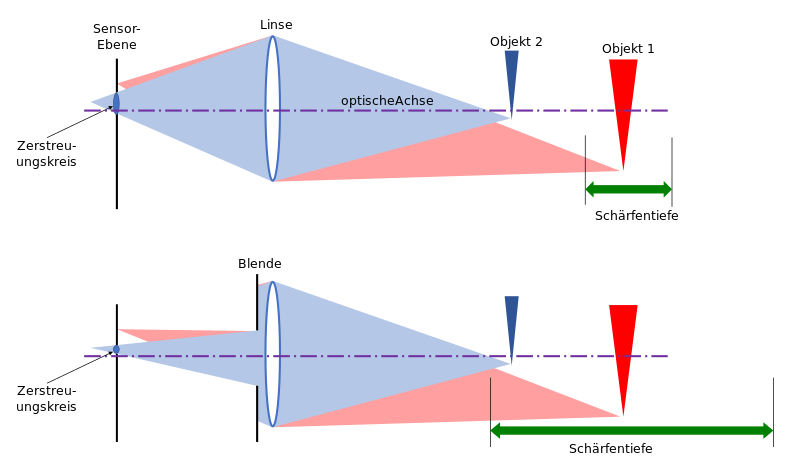
\includegraphics[width=0.7\textwidth]{figures/schaerfentiefe.png}
\end{defi}

\begin{defi}{Zerstreuungskreis}
    % TODO: https://de.wikipedia.org/wiki/Zerstreuungskreis 
    \emph{Zerstreuungskreise} entstehen in der Fotografie bei Unschärfe im Bild, also wenn die Projektion eines Punktes eines Motivs vor beziehungsweise hinter der Projektionsebene liegt oder wenn durch Beugung ein zu projizierender Lichtpunkt unscharf als Beugungsscheibchen abgebildet wird.

    Diese beiden Effekte, die eine Unschärfe hervorrufen, sind bei veränderter Eintrittspupille gegenläufig, so dass sich bei einer bestimmten Blende, der sogenannten kritischen Blende, eine minimale Unschärfe und somit ein maximales Auflösungsvermögen ergibt.

    \centering
    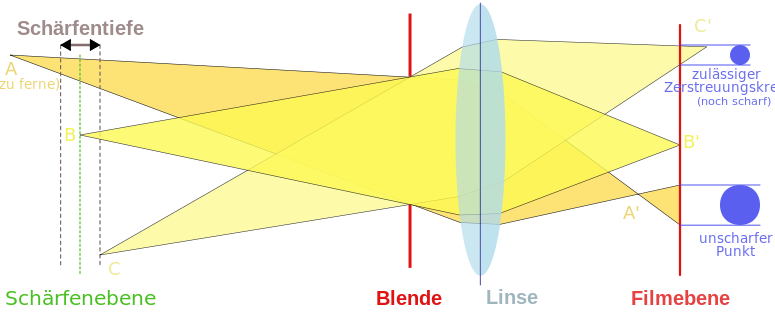
\includegraphics[width=0.6\textwidth]{figures/zerstreuungskreis.png}
\end{defi}

\begin{defi}{Bildkreis}
    % TODO: https://de.wikipedia.org/wiki/Bildkreis 
    Der \emph{Bildkreis} beschreibt in der Fotografie jenen Bereich, den ein Objektiv bildseitig ausleuchten kann. Damit der Film oder der Sensor vollständig beleuchtet wird, muss der Durchmesser des Bildkreises mindestens so groß sein wie die Diagonale des Film- bzw. Sensorformats.

    Der mindestens erforderliche Bildkreisdurchmesser $D$ eines Objektivs errechnet sich als Diagonale des Negativs bzw. rechteckigen Sensors (Breite $B$ und Höhe $H$) nach dem Satz des Pythagoras mit der Formel
    \[
        D = \sqrt{B^2 + H^2}
    \]
\end{defi}

\begin{defi}{Bildwinkel}
    Der \emph{Bildwinkel} definiert den Bereich des Gegenstandsraums, der durch das Objektiv und durch die Ränder des Sensorformats begrenzt wird.

    Außer durch das Bildformat -- Höhe $H$, Breite $B$ bzw. Diagonale $D$ des Bilds -- wird der Bildwinkel $\alpha$ im Wesentlichen nur noch durch die aktuelle Brennweite $f$ des Kameraobjektivs bestimmt.
    Die nachstehende Formel liefert dementsprechend den diagonalen Bildwinkel bei Einstellung des Objektivs auf \enquote{unendlich}:
    \[
        \alpha_d = 2 \cdot \arctan \left( \frac{D}{2 \cdot f} \right)
    \]
    Bei Abbildung näherer Gegenstände dagegen wird die Bildweite $B$ größer als $f$, wodurch sich der Bildwinkel $\alpha$ entsprechend verkleinert.

\end{defi}

\begin{defi}[Kamera]{Sensor}
    % TODO: https://de.wikipedia.org/wiki/Digitalkamera#Bildwandlung 
    Wie bei einer Analogkamera wird das einfallende Licht mit einem Objektiv gesammelt und auf die Filmebene, in Fall einer Digitalkamera auf den \emph{Sensor}, scharfgestellt (fokussiert).

    Der Sensor kann entweder ein Flächensensor oder (selten) ein Zeilensensor sein. Der Flächensensor steht fest in der Filmebene, er registriert gleichzeitig das gesamte Bild. Zeilensensoren werden in Scannerkameras eingesetzt, die nach dem Scannerprinzip funktionieren, das heißt, sie arbeiten ähnlich wie ein Flachbettscanner und tasten das Bild zeilenweise ab: Der Zeilensensor wird mittels Antriebs über die Filmebene gefahren, dabei wird Zeile um Zeile erfasst.

    Die Erfassung der drei Grundfarben kann gleichzeitig im selben Sensor geschehen, der dann für jeden Vollfarb-Pixel drei Subpixel besitzt.
    Die Grundfarben können jedoch auch räumlich getrennt erfasst werden, indem z. B. ein System aus halbdurchlässigen Spiegeln das einfallende Licht auf drei getrennte Sensoren für die drei Grundfarben verteilt.
    Als dritte Möglichkeit können die Grundfarben zeitlich getrennt erfasst werden:
    Gleichzeitig (One-shot-Kameras) oder nacheinander (Three-Shot-Kameras), wobei dann vor jeder Erfassung ein anderer Farbfilter vorgeschaltet wird.
\end{defi}

\begin{defi}[Kamera!Sensor]{Kontrastumfang}
    TODO
\end{defi}

\begin{bonus}[Kamera!Sensor]{Räumliche Diskretisierung}
    TODO
\end{bonus}

\begin{bonus}[Kamera!Sensor]{Funktionsweise}
    TODO
\end{bonus}

\begin{defi}[Kamera!Sensor]{Abtastung}
    TODO
\end{defi}

\begin{defi}[Kamera!Sensor]{Quantisierung}
    TODO
\end{defi}